
\documentclass[fleqn,12pt]{article}

\usepackage[margin=15mm]{geometry}
\usepackage[utf8]{inputenc}
\usepackage[bulgarian]{babel}
\usepackage[unicode]{hyperref}
\usepackage{amsfonts}
\usepackage{amssymb}
\usepackage{enumitem, hyperref}
\usepackage{upgreek}
\usepackage{indentfirst}
\usepackage{graphicx}
\graphicspath{ {./diagrams/} }

\title{Тема 14\\ Софтуерно инженерство и неговото място като дял от знанието. Софтуерен процес и модели на софтуерни процеси. Концепция за многократна употреба.}

\author{v0.5}
\date{26 юни 2021}

\begin{document}

\maketitle

\tableofcontents

\clearpage

\section{Софтуерното  инженерство}
\subsection{Какво  е  софтуер?}
Един софтуерът може да се определи като съвкупност от:
\begin{itemize}
	\item Инструкции (програми), които при изпълнение осигуряват желаните характеристики, функционалностти и производителност
	\item Структури от данни, които дават възможност на програмите да манипулират информацията адекватно
	\item Документация, описваща работата и използването на програмите
\end{itemize}

Софтуера се обособява, чрез следните характеристики:
\begin{itemize}
	\item Софтуера се разработва, не се произвежда
	\item Софтуера не се износва
	\item Софтуера е сложен и притежава голямо ниво на абстрактност
\end{itemize}

\subsection{Видове  софтуер}
Имаме няколко вида софтуер:
\begin{itemize}
	\item Системен софтуер
	\item Приложен софтуер
	\item Научен софтуер
	\item Вграден софтуер
	\item Продуктова линия
	\item Уеб приложения
	\item Изкуствен интелект
	\item Системи от системи
	\item Наследен софтуер
\end{itemize}

\subsection{Същност и обхват на софтуерното инженерство}
Инженерството се състой от анализ, проектиране, конструиране, верифициране и управление на технически (или социални) единици. Софтуерното инженерство е дисциплина, която се занимава с всички аспекти на проектирането и разработката на \textbf{висококачествен} софтуер.

Софтуерните инженери би трябвало да възприемат в своята работа систематизиран и организиран подход на разработка. Също така трябва да използват подходящи средства в зависимост от решавания проблем, съществуващите ограничения и начичните ресурси

Ако един софтуер се разработва с цел решаването на даден проблем, то можем да кажем, че софтуерното инженерство се занимава с:
\begin{itemize}
	\item Разбирането и анализирането на проблема
	\item Намиране на решение за проблема - конструиране от части, които засягат различни аспекти на проблема. Този процес се нарича синтез.
	\item Решаване на проблема с използване на различни методи, парадигми, процедури и парадигми
\end{itemize}

\section{Софтуерен  процес}

Софтуерния процес е последователност от стъпки включващи дейности, ограничения и ресурси, които се следват за създаването на продукт или система в даден срок и с високо качество.

\subsection{Фази и  основни  дейности}
\subsubsection{Фази на софтуерния процес:}
\begin{itemize}
	\item Анализ и дефиниране на изискванията
	\item Проектиране на системата
	\item Проектиране на програмата
	\item Писане на програмата
	\item Тестване на единици (unit testing)
	\item Интеграционно тестване (integration testing)
	\item Тестване на системата
	\item Доставяне на системата
	\item Поддръжка
\end{itemize}

\subsubsection{Основни дейности на софтуерния процес:}
\begin{itemize}
	
	\item Комуникация
	\begin{itemize}
		\item събиране и разбиране на изисквания за функционалността на софтуера и за ограниченията вурху разработката му
	\end{itemize}
	
	\item Планиране
	\begin{itemize}
		\item Създава се план за бъдещата работа по разработката на софтуера
		\item Описват се рисковете, необходимите ресурси, графика и крайните продукти
	\end{itemize}
	
	\item Моделиране - има 2 части: Анализ и проектиране
	\begin{itemize}
		\item Анализ:
		\begin{itemize}
			\item Работни задачи: Събиране на изисквания, Уточняване, Договаряне, Специфициране и Валидиране
			\item Работни продукти: Модел на анализа и Спецификация на изискванията
		\end{itemize}
		
		\item Проектиране:
		\begin{itemize}
			\item Работни задачи: Дизайн на данните, архитектурата, интерфейсите и нивото на компонентите.
			\item Работни продукти: Модел и спецификация на дизайна
		\end{itemize}
	\end{itemize}

	\item Конструиране
	\begin{itemize}
		\item Генериране на код:
		\item Тестване:
		\begin{itemize}
			\item тестване на самостоятелни компоненти
			\item тестване на интегрираната система (модулите + подсистемите + системата)
			\item потребителско (бета) тестване
		\end{itemize}
	\end{itemize}

	\item Внедряване
	\begin{itemize}
		\item Софтуерът се предоставя на клиента:
		\item Клиентът оценява продукта като дава обратна връзка и препоръки:
	\end{itemize}
\end{itemize}

\subsubsection{Допълнителни дейности на софтуерния процес:}
\begin{itemize}
	\item Следене и управление на софт. продукт
	\item Управление на риска
	\item Осигуряване на качеството
	\item Формални технически прегледи
	\item Измерване на системата
	\item Управление на софтуерната конфигурация
	\item Управление на повторното използване
	\item Подготовка и генериране на работни продукти
\end{itemize}

\subsection{Модели на софтуерния процес}
Един модел представлява опростено описание на начина на разработка на софтуера, представено от определена гледна точка. Те биват няколко вида:

\begin{itemize}
	\item Описателни модели - как се разработва софтуера
	\item Предписателни модели - как би трябвало да се разработва софтуера.
	\begin{itemize}
		\item те дефинират специално множество от дейности, задачи, milestone-ове и работни продукти, които са необходими за създаването на софтуер с високо качество.
	\end{itemize}
\end{itemize}

\subsection{Езици за  моделиране}
Език за моделиране на процеси е език, адаптиран или създаден с цел представянето на процеси. Те се използват за представяне по прецизен и изчерпателен начин следните характеристики на софтуерния процес:
 
\begin{itemize}
	\item Дейностите, които трябва да се извършат, за да се постигнат целите на процеса
	\item Ролите на хората, участващи в процеса
	\item Структурата и същността на артефактите, които се създават и поддържат
	\item Средствата, които се използват
\end{itemize}

\subsection{Шаблони за описание}
Шаблон е описание на общо решение на общ проблем, на базата на което може да се извлече детайлно решение на специфичен проблем.
Шаблон за описание на процес представлява структурирано описание на процес, което е метод за описание на важните характеристики на софтуерния процес. Шаблоните могат да бъдат дефинирани на различни нива на абстракция. Важна характеристика за шаблоните е, че описва какво да се направи, но не \textbf{как} да се направи.

\section{Сравнителен анализ на описателни модели на софтуерен процес}
\subsection{Модел на водопада}
Най-стария метод за разработване. Предлага последователен подход към разработването на софтуер.

\leavevmode \newline
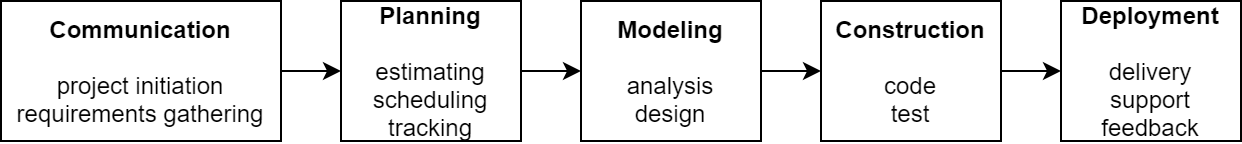
\includegraphics[width=\textwidth]{waterfall}
\leavevmode \newline

Предимства и недостатъци:
\begin{description}
	\item \textbf{+} ясно разграничен процес, който е лесен за разбиране.
	\item \textbf{+} всяка стъпка завършва със създаването на документация
	\item \textbf{+} всяка дейност трябва да бъде завършена, преди да се премине към следващата
	\item \textbf{+} ясно дефинирани входове, изходи и интерфейси между отделните стъпки
	\item \textbf{+} ясно дефинирани роли на разработчиците
	\item \textbf{---} реални проекти рядко следват последователния поток на разработване
	\item \textbf{---} трудно е за потребителя да формулира всичките си изисквания в началото, без да са нужни промени нататък.
	\item \textbf{---} клиентът трябва да е търпелив
	\item \textbf{---} разделянето на проекта на отделни етапи не е гъвкаво
	\item \textbf{---} трудно е да се реагира на променящите се изисквания на клиента
\end{description}

\subsection{Модел на бързата разработка}
Моделът на бързата разработка, познат също като RAD, e високоскоростен вариант на модела на водопада. Главната идея е системата да се раздели на няколко подсистеми и няколко софтуерни екипа да работят по отделните подсистеми паралелно.

\leavevmode \newline
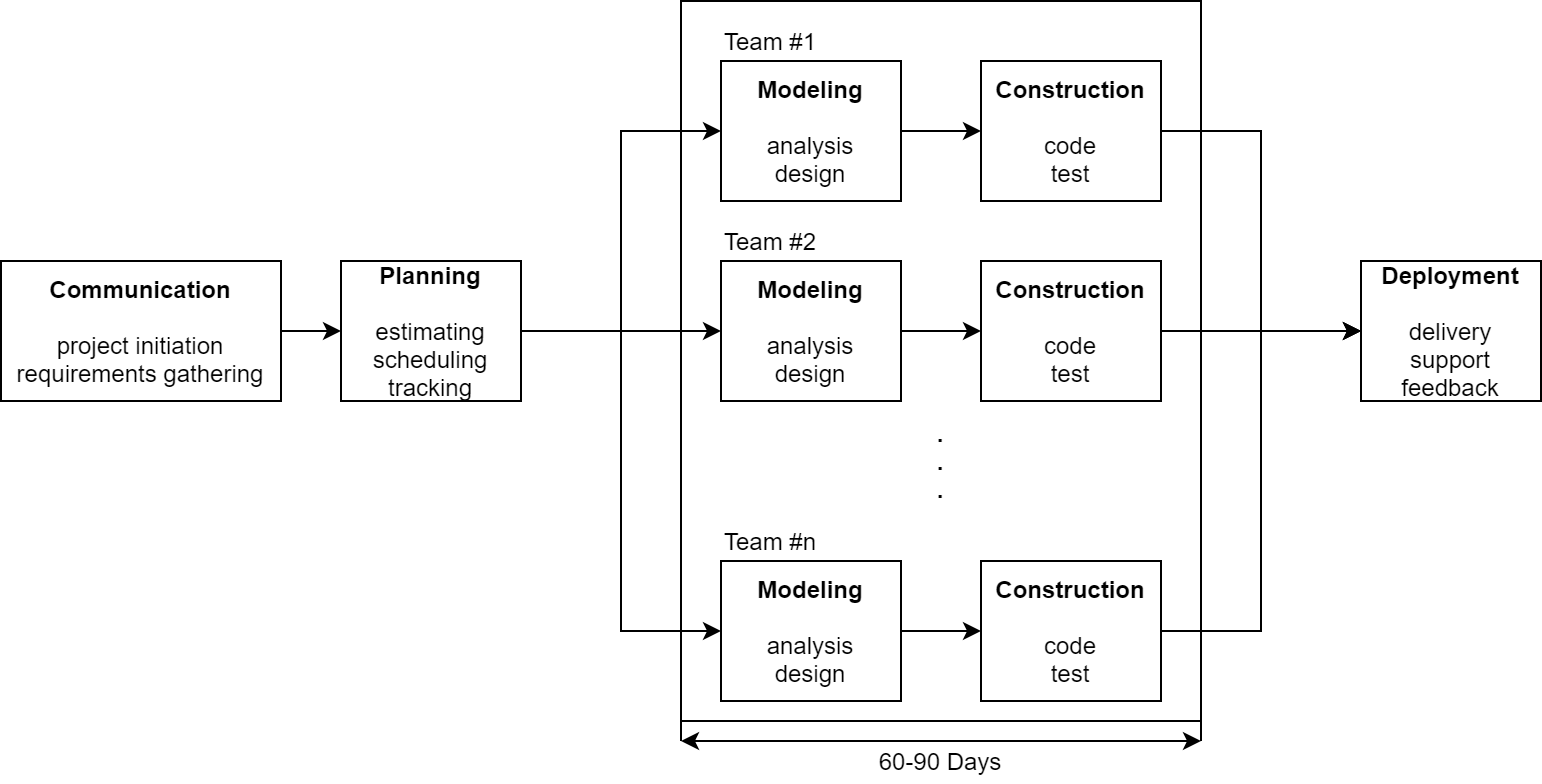
\includegraphics[width=\textwidth]{RAD}
\leavevmode \newline

Предимства и недостатъци:
\begin{description}
	\item \textbf{+} използват се вече съществуващи софт. компоненти, които се интегрират
	\item \textbf{+} използват се средства за автоматично генериране на код
	\item \textbf{---} за големи приложения, подлежащи на разделяне на модули, са нужни значителни човешки ресурси
	\item \textbf{---} моделът не е подходящ, ако функционалността на системата не може да бъде подходящо разделена в отделни модули
	\item \textbf{---} моделът не е подходящ, ако производителността е важна за системата
	\item \textbf{---} моделът не е подходящ, ако се разчиат на нови или недостатъчно усвоени технологии
\end{description}

\subsection{Еволюционен модел}
При еволюционните модели системата не се доставя като едно цяло, а вместо това се разработва на "стъпки" и се доставя на части, през целия процес на разработка. Методът ефективно комбинира елементи от модела на водопада, но са приложени на отделни стъпки. Така се доставя цялата система още в началото, като някои от функционалностите са в примитивна форма.

Предимства и недостатъци:
\begin{description}
	\item \textbf{+} клиентът може да използва системата, преди да е напълно завършена
	\item \textbf{+} първите версии на системата могат да служат като прототип, за да помогнат за изяснясняване на изискванията
	\item \textbf{+} рискът за неуспех на целия проект е по-малък
	\item \textbf{+} функционалностите с най-висок приоритет са тествани най-много
	\item \textbf{---} необходимо е клиентите да участват активно, може да доведе до закъснения
	\item \textbf{---} слаба комуникацията между клиентите и разработчиците може да доведе до проблеми  
	\item \textbf{---} неформалните заявки за подобрения могат да доведат до объркване
	\item \textbf{---} този модел може да доведе до "scope creep" (бавно и постепенно разширение на обхвата на проекта)
\end{description}

\subsection{Прототипен модел}
Прототипните модели биват 2 вида:

\begin{itemize}
	\item Еволюционен - целта е да се достави работеща система, като финалния продукт е бил развит от някакъв прототип
	\item Изхвърлен прототип - ползва се за подпомагане специфицирането на изискванията към софтуера, след което в повечето случай 
\end{itemize}

Подхода при този модел е да се създаде минимална версия на системата, която изпълнява ограничено подмножество функционалности. Целта е да се демонстрират функционалности, които ще са включват в системата. Прилага се при системи, където изискванията и дизайнът не са достатъчно ясни. Често се използва вече съществуващи системи или компоненти за демонстрирането.

Предимства и недостатъци:
\begin{description}
	\item \textbf{+} помага при изясняването на потребителските изисквания и дизайна
	\item \textbf{+} може да се използва самостоятелно, и в комбинация с други модели
	\item \textbf{---} възможно е да се използват значителни ресурси, а прототипа да не може да удолетвори очакванията
	\item \textbf{---} крайната система може да се окаже зле проектирана, ако е била надграждана на прототипа.
	\item \textbf{---} не е подходящ при системи, където проблема е добре разбран или интерфейсът е ясен и прост
\end{description}

\subsection{Спираловиден модел}
Спираловидния модел е еволюционен модел, който съчетава прототипния модел и модела на водопада. Модела е цикличен, като на всеки цикъл се извършват дейностите на модела на водопада и на края на цикъла се преразглеждат и променят изискванията и се преминава към следващ цикъл.

\leavevmode \newline
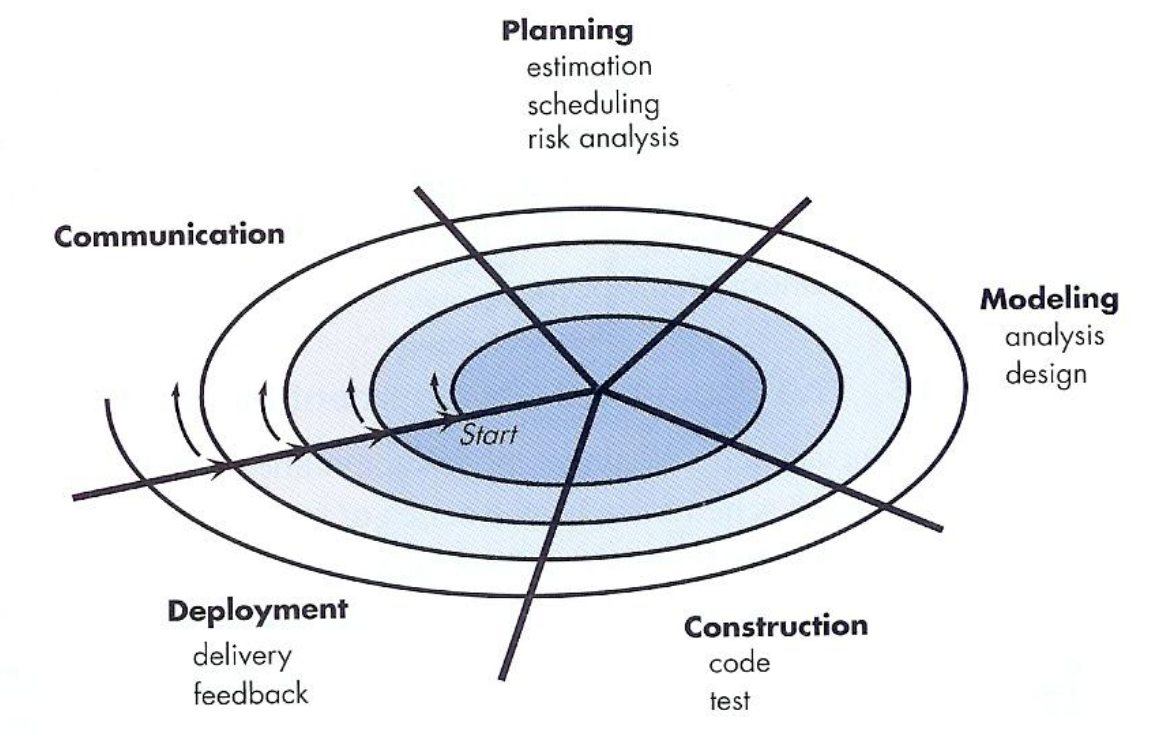
\includegraphics[width=\textwidth]{spiral}
\leavevmode \newline

Предимства и недостатъци:
\begin{description}
	\item \textbf{+} помага при разработването на огромни системи
	\item \textbf{+} може да се адаптира и приложи през целия жизнен цикъл на софтуера
	\item \textbf{---} трудно е да се убедят клиентите, че процесът не е безкраен
	\item \textbf{---} изисква се участието на разработчици, компетентни в оценяването на рисковете
	\item \textbf{---} ако има основен риск, който е останал неоткрит, той може да доведе до неуспех
\end{description}

\section{Концепция за многократна употреба}
В повечето инженерни дисциплини системите се проектират чрез композиране на вече съществуващи компоненти.

Ползи от многократната употреба
\begin{itemize}
	\item Увеличава се предвидимостта по отношение на качеството и процеса на разработка.
	\item Увеличава се скоростта на разработка
	\item По-ефективно ползване на ресурсите
	\item По-лесно придържане към стандартите
	\item Около 15\% от кода, който се пише е за нови цели, тоест до 85\% от кода може да се преизползва
	\item Няма друг начин да се създават големи приложения
\end{itemize}

Има 2 подхода за многократна употреба: първия е базиран на създаване на програмни единици, а другия е базиран на съществуващи програмни единици.

\subsection{Многократна употреба, базирана на съществуващи програмни единици}

Има няколко вида:
\begin{itemize}
	\item COTS (Component-Off-The-Shelf) продукти
	\begin{description}
		\item \textbf{+} цели приложения, предлагащи API
		\item \textbf{+} приложими в широк кръг области
		\item \textbf{+} по-бърза разработка и по-ниска цена
		\item \textbf{---} липса на контрол върху функционалността и производителността
		\item \textbf{---} интеграцията може да се окаже трудна
		\item \textbf{---} липса на контрол върху развитието и новите версии на продуктите
		\item \textbf{---} недостатъчна поддръжка от производителите на COTS
	\end{description}
	\item Компонентно-базирано разработване
	\begin{itemize}
		\item компонентите предоставят една и съща услуга, без значение от платформата или езикът
		\item независими самостоятелно изпълними единици
		\item ползват входни и изходни интерфейси за да се използват
		\item може да се каже, че COTS е частен случай на компонентно-базирано разработване
	\end{itemize}
	\item Аспектно ориентирано разработване
	\begin{itemize}
		\item то засяга така нареченото разделяне на функциите
		\item припокриващата функционалност се разработва като аспекти, които динамично се вмъкват в програмата
		\item често е трудно те да се отделят чрез стандартните методи на проектиране.
	\end{itemize}
	\item Архитектура, ориентирана към услуги
	\begin{itemize}
		\item основава се на идеята за услуги, достъпвани "отвън"
		\item уеб-услугата е стандартизиран подход за осигуряване на някаква функционалност, достъпна чрез интернет
		\item ползват се няколко стандарта:
		\begin{itemize}
			\item SOAP - Simple Object Access Protocol
			\item WSDL - Web Services Description Language
			\item UDDI - Universal Description, Discovery and Integration
		\end{itemize}
	\end{itemize}
\end{itemize}

\subsection{Многократна употреба, базирана на създаване на програмни единици}

Има няколко вида:
\begin{itemize}
	\item Шаблони за проектиране (Design Patterns)
	\begin{itemize}
		\item използва някакво абстрактно знание за дадена задача и решението ѝ
		\item описва задачата и най-съществените моменти от решението
		\item предполага възможност за прилагане в различни ситуации
	\end{itemize}
	\item Програмна генерация
	\begin{itemize}
		\item използват вече дефинирани шаблони и алгоритми, които са вградени в генератора и могат да се параметризират
		\item програмата се генерира автоматично
		\item програмната генерация е възможна, когато може да се дефинира съответствие между понятията от приложната област и кода
		\item ефективен метод за разработка
		\item приложимостта му е в ограничен набор приложни области
		\item по-лесно от стандартните компонентни подходи
	\end{itemize}
\end{itemize}

\end{document}
